\section{Auswertung}
\label{sec:Auswertung}

\subsection{Bestimmung der Apparatenkonstante}
\label{sec:Apparatenkonstante}
Um die Apparatenkonstante zu bestimmen, werden die Dichten der Kugeln benötigt.
Die Messwerte der Massen und Radien der beiden Kugeln sind in Tabelle \ref{tab:MasseundDichte} zu finden.
Die Radien und Massen bestimmen sich zu
\begin{align*}
  r_{\symup{Gr}} &= (7,86 \pm 0,04)\cdot 10^{-3} \,\si{\meter}\\
  m_{\symup{Gr}} &= (4,54 \pm 0,01) \cdot 10^{-3} \,\si{\kilo\gram}\\
  r_{\symup{Kl}} &= (7,64 \pm 0,11)\cdot 10^{-3} \,\si{\meter}\\
  m_{\symup{Kl}} &= (4,44 \pm 0,02) \cdot 10^{-3} \,\si{\kilo\gram}.\\
\end{align*}

Aus () ergibt sich für die Dichten
\begin{align*}
  \rho_{\symup{Gr}} &= (2232 \pm 34) \,\frac{\si{\kg}}{\si{m^3}}  \\
  \rho_{\symup{Kl}} &= (2380 \pm 10) \,\frac{\si{\kg}}{\si{m^3}}. \\
\end{align*}

\begin{table}
  \centering
  \caption{Messdaten der Massen und Radien der beiden Kugeln.}
  \label{tab:MasseundDichte}
  \begin{tabular}{c c c c}
    \toprule
    $r_{\symup{Gr}}/10^{-3}\,\unit{\meter}$ & $m_{\symup{Gr}}/10^{-3}\,\unit{\kilo\gram}$ & $r_{\symup{Kl}}/10^{-3}\,\unit{\meter}$ & $m_{\symup{Kl}}/10^{-3}\,\unit{\kilo\gram}$ \\
    \midrule
    7,90 & 4,54 & 7,75 & 4,46 \\
    7,80 & 4,56 & 7,55 & 4,46 \\
    7,85 & 4,54 & 7,55 & 4,43 \\
    7,90 & 4,54 & 7,80 & 4,42 \\
    7,85 & 4,54 & 7,55 & 4,43 \\
    \bottomrule
  \end{tabular}
\end{table}
Weiterhin werden noch die Fallzeiten der beiden Kugeln im Viskosimeter benötigt.
Die Fallzeiten der kleinen und der großen Kugel sind in Tabelle \ref{tab:Fallzeit} angegeben. Aus den Messwerten ergibt sich für die Fallzeiten
\begin{align*}
  t_{\symup{Kl}} &= (12,04 \pm 0,18)\,\unit{\second} \\
  t_{\symup{Gr}} &= (39,7 \pm 0,39)\,\unit{\second}. \\
\end{align*}

\begin{table}
  \centering
  \caption{Fallzeiten der Kugeln.}
  \label{tab:Fallzeit}
  \begin{tabular}{c c | c c}
    \toprule
    $t_{\symup{Kl}}/\unit{\second} $ & $ $ & $t_{\symup{Gr}}/\unit{\second}$ & $ $ \\
    \midrule
    12,28 & 12,12 & 40,17 & 39,52 \\
    12,06 & 12,13 & 40,17 & 39,60 \\
    11,94 & 11,88 & 39,27 & 39,43 \\
    11,97 & 11,97 & 39,67 & 39,49 \\
    12,12 & 12,09 & 39,67 & 38,92 \\
    12,12 & 12,47 & 39,55 & 39,09 \\
    12,13 & 12,15 & 39,40 & 40,11 \\
    11,87 & 12,06 & 39,57 & 40,17 \\
    11,87 & 12,06 & 40,52 & 39,99 \\
    11,59 & 11,84 & 39,85 & 39,88 \\
    \bottomrule
  \end{tabular}
\end{table}

Nun wird mit Hilfe der Fallzeitwerte der kleinen Kugel die Viskosität von Wasser bei Raumtemperatur bestimmt. Dabei werden
\begin{align*}
  K_{\symup{Kl}} &= 7,64\cdot 10^{-8} \,\frac{\unit{\pascal}\cdot\unit{\meter^3}}{\unit{\kilo\gram}} \\
  \rho_{\symup{Fl}} &= 998,2\,\frac{\unit{\kilo\gram}}{\unit{\meter^3}}
\end{align*}
verwendet. $K_{\symup{Kl}}$ ist die angegeben Appartenkonstante für die kleine Kugel \cite{anleitung107}  und $\rho_{\symup{Fl}}$
die Dichte von Wasser bei Raumtemperatur \cite{waterdensity}. Aus (\ref{eqn:etaK}) ergibt sich für die Viskosität des Wassers bei Raumtemperatur
\begin{align*}
  \eta_{\symup{RT}} = (1,27 \pm 0,02)\cdot 10^{-3} \,\unit{\pascal}\cdot\unit{\second}.
\end{align*}
Durch Umstellen von (\ref{eqn:etaK}) und einsetzen der Werte ergibt sich nun
\begin{align*}
  K_{\symup{Gr}} = (2,59 \pm 0,09)\cdot 10^{-8}\,\frac{\unit{\pascal}\cdot\unit{\meter^3}}{\unit{\kilo\gram}}
\end{align*}
für die Apparatenkonstante der großen Kugel.

\subsection{Temperaturabhängigkeit der Viskosität}
\label{sec:TempVisk}
Nun kann mit (\ref{eqn:etaK}) die Viskosität für unterschiedliche Temperaturen berechnnet werden. Die Werte für die Fallzeit der Kugel und Temperatur und Dichte \cite{waterdensity}
des Wassers sind in Tabelle \ref{tab:Temp} angegeben. 

\begin{table}
  \centering
  \caption{Messdaten zur Bestimmung der Temperaturabhängigkeit der Viskosität.}
  \label{tab:Temp}
  \begin{tabular}{c c c c | c c c c}
    \toprule
    $T/\unit{\kelvin}$ & $t/\unit{\second}$ & $\rho_{\symup{Fl}}/\frac{\unit{\kilo\gram}}{\unit{\meter^3}}$ & $\eta/10^{-3}\unit{\pascal}\cdot \unit{\second}$ & $T/\unit{\kelvin}$ & $t/\unit{\second}$ & $\rho_{\symup{Fl}}/\frac{\unit{\kilo\gram}}{\unit{\meter^3}}$ & $\eta/10^{-3}\unit{\pascal}\cdot \unit{\second}$ \\
    \midrule
    293,15 & 39,90 & 998,21 & 1,276 & 308,15 & 28,33 & 994,03 & 0,909 \\
    293,15 & 39,27 & 998,21 & 1,256 & 308,15 & 28,22 & 994,03 & 0,906 \\
    293,15 & 39,61 & 998,21 & 1,267 & 311,15 & 27,77 & 992,97 & 0,892 \\
    293,15 & 38,93 & 998,21 & 1,245 & 311,15 & 27,43 & 992,97 & 0,881 \\
    296,15 & 37,92 & 997,54 & 1,214 & 311,15 & 27,76 & 992,97 & 0,892 \\
    296,15 & 36,39 & 997,54 & 1,165 & 311,15 & 27,35 & 992,97 & 0,879 \\
    296,15 & 36,94 & 997,54 & 1,182 & 314,15 & 26,48 & 991,83 & 0,851 \\
    296,15 & 36,61 & 997,54 & 1,172 & 314,15 & 25,02 & 991,83 & 0,805 \\
    299,15 & 35,61 & 996,79 & 1,140 & 314,15 & 26,09 & 991,83 & 0,839 \\
    299,15 & 34,52 & 996,79 & 1,106 & 314,15 & 25,36 & 991,83 & 0,815 \\
    299,15 & 35,11 & 996,79 & 1,124 & 317,15 & 24,61 & 990,63 & 0,792 \\
    299,15 & 34,49 & 996,79 & 1,105 & 317,15 & 24,40 & 990,63 & 0,785 \\
    302,15 & 32,74 & 995,95 & 1,049 & 317,15 & 24,25 & 990,63 & 0,781 \\
    302,15 & 31,61 & 995,95 & 1,013 & 317,15 & 24,38 & 990,63 & 0,785 \\
    302,15 & 32,33 & 995,95 & 1,036 & 320,15 & 23,42 & 989,37 & 0,755 \\
    302,15 & 31,83 & 995,95 & 1,020 & 320,15 & 22,80 & 989,37 & 0,735 \\
    305,15 & 30,80 & 995,03 & 0,988 & 320,15 & 23,05 & 989,37 & 0,743 \\
    305,15 & 30,27 & 995,03 & 0,971 & 320,15 & 22,95 & 989,37 & 0,739 \\
    305,15 & 30,52 & 995,03 & 0,979 & 323,15 & 21,55 & 988,04 & 0,695 \\
    305,15 & 30,22 & 995,03 & 0,969 & 323,15 & 21,71 & 988,04 & 0,700 \\
    308,15 & 28,33 & 994,03 & 0,909 & 323,15 & 21,58 & 988,04 & 0,696 \\
    308,15 & 28,80 & 994,03 & 0,924 & 323,15 & 22,08 & 988,04 & 0,712 \\
    \bottomrule
  \end{tabular}
\end{table}

Durch Auftragen von $ln(\eta)$ gegen $\frac{1}{T}$ in Abbildung \ref{fig:plot} lassen sich mit Hilfe von Linearer Regression die Konstanten $A$ und $B$
aus der Andradeschen Gleichung (\ref{eqn:Andrad}) bestimmen.
\begin{align*}
  \eta(T) &= A \, \exp{\left(\frac{B}{T}\right)} \\
  \iff ln(\eta) &= ln(A) + ln(\frac{B}{T})
\end{align*}
Da für jede Temperatur viermal gemessen wurde, sind die Viskositätswerte gemittelt.

\begin{figure}
  \centering
  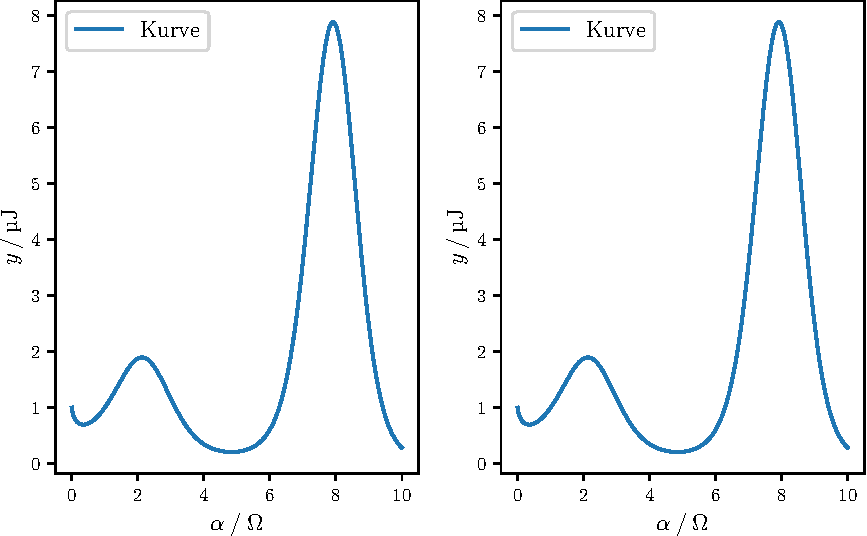
\includegraphics{plot.pdf}
  \caption{Ausgleichsgerade zur Bestimmung der Konstanten der Andradeschen Gleichung.}
  \label{fig:plot}
\end{figure}

Insgesamt ergibt sich
\begin{align*}
  A &= (2,0 \pm 0,5)\cdot 10^{-6}\,\unit{\pascal}\cdot \unit{\second}\\
  B &= (1895 \pm 71)\,\unit{\kelvin}
\end{align*}
Abschließend wird überprüft, ob es sich um eine laminare oder turbulente Strömung handelt. Dies geschieht mit Hilfe der Reynoldszahl, die einmal für die kleine und
einmal für die große Kugel bestimmt wird und dann mit der kritischen Reynoldszahl abgeglichen wird. In Gleichung (\ref{eqn:Reynoldzahl}) wird $\bar{v} = \frac{x}{t}$
und $d = 2r$ eingesetzt. Die REynoldszahlen der kleinen und der großen Kugel ergeben sich zu
\begin{align*}
  Re_{\symup{Kl}} &= 49,9 \pm 1,3\\
  Re_{\symup{Gr}} &= 15,56 \pm 0,30.
\end{align*}
Da die Reynoldszahlen kleiner als die kritische Reynoldszahl ist, sind die Strömungen laminar.